\subsubsection{NXT Servomotor (ID: 53787)}
\begin{figure}[H]
  \centering
  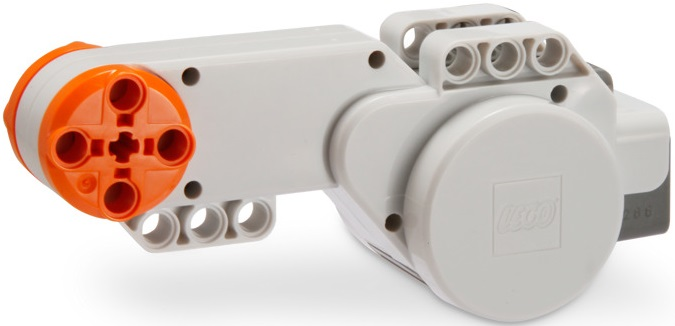
\includegraphics[width=3cm]{images/techAnalysis/LegoNXT2Servomotor.jpg}
  \caption{LEGO MINDSTORMS NXT 2.0 servomotor \cite{BrickOWl-figure-NXT2-Servo}}\label{fig:sssec:nxtServomotor}
\end{figure}
As previously described, the NXT 2.0 was the predecessor to the EV3 within the LEGO MINDSTORMS universe, this also applies to the NXT servomotor, which was the motor for the NXT 2.0.
This servomotor, shown in \autoref{fig:sssec:nxtServomotor}, like the EV3 large servomotor, allows for precise control to a single degree of accuracy, with its built-in rotation sensor.
It works on both the LEGO MINDSTORMS EV3 brick and the LEGO MINDSTORM NXT 2.0 brick by default, and is powered and connected through its RJ12 port, like the EV3 large servomotor \cite{lego_lego_EV3NXTCompatibility}.
It is tested by Philippe Hurbain, an engineer who was one of the authors of the book "Extreme NXT", to run at a maximum of just above 160rpm \cite{gasperi_extreme_2009} \cite{hurbain_nxt_nodate}.
\cite{lego_mindstorms_2009}
